\chapter{Introducción}

En el presente trabajo se realiza el análisis estadístico de texto, empleando como fuente a los comentarios de la transmisión en vivo del primer debate presidencial, realizado el día 7 de abril del 2024; los comentarios presentan una estructura lingüística mal estructurada, de igual forma, se identifican Emojis entre apalabras o comentarios completos a partir de los mismos.\\


\section{Primer objetivo}\\
 Generar información estadística que nos permita visualizar los elementos característicos, que forman parte de los comentarios, como son, la frecuencia palabras, votos a los comentarios (Top 10 de votos), frecuencias de participación en los comentarios (Top 10 de Usuarios) y la relación entre los votos y las replicas.\\

\section{Segundo objetivo}\\
 Realizar una comparativa entre el numero de menciones y la estadística de intención de voto previo a este debate, a modo de comparación estadística entre la expresión del nombre de los candidatos en los comentarios y la intención de voto documentada hasta ese momento.\\
   


\chapter{descripción de los datos}

Del total de datos unicamente consideraremos el siguiente conjunto de columnas:\\

\begin{itemize}
	\item ID: identificador de comentario
	\item text : Comentario del Usuario.
	\item author : Nombre de usuario que realiza el comentario.
	\item votes : numero de votos recibidos 
	\item replies : número de replicas en los comentarios.\\
\end{itemize} 

Se identifican un total de 4307 comentarios publicados en el video de Youtube (URL: https://www.youtube.com/watch?v=kZaucITWv00&t=18s), de los cuales 2352 representan algun comentario sin estructura textual o verbal, correspondiendo a signos puntuales o emojis.\\

En total tenemos un conjunto de 1955 participaciones con algún tipo de comentario textuales ademas de Emojis, en el cuadro \ref{tab:T1} podemos observar una muestra representativa del conjunto de datos. \\

\begin{table}[H]
	\centering
	\resizebox{\textwidth}{!}{%
		\begin{tabular}{ccccc}
			\rowcolor[HTML]{9B9B9B} 
			\textbf{ID}             & \textbf{text}                                      & \textbf{author}         & \textbf{votes}          & \textbf{replies}        \\
			0                       & El reloj debió verse en todo momento, para ten...  & @celinaramirez6363      & 394                     & 16.0                    \\
			1                       & Me uno a exigir que pongan los relojes de los ...  & @puellacodicum8569      & 555                     & 19.0                    \\
			2                       & Me parece muy bien cómo contestó Maynes, fue d...  & @alondrareal8518        & 79                      & NaN                     \\
			\multicolumn{1}{l}{...} & \multicolumn{1}{l}{...}                            & \multicolumn{1}{l}{...} & \multicolumn{1}{l}{...} & \multicolumn{1}{l}{...} \\
			1953                    & Maynes, palero de Claudia \#CrimesAgainstHumani... & @yamerosolitario2       & 0                       & NaN                     \\
			1954                    & Xóchitl Presidente                                 & @marcoantonioarroyo952  & 0                       & NaN                     \\
			1955                    & Cuánto dinero les pagaste por esos reconocimie...  & @maru641                & 0                       & NaN                    
		\end{tabular}%
	}
	\caption{}
	\label{tab:T1}
\end{table}

A partir de los datos podemos generar algunos elementos estadísticos interesantes del conjunto, por ejemplo el top 10 de mensajes por usuario, lo que nos indica la participación dentro de los comentarios, identificando los usuarios mas activos e identificar posteriormente su inclinación política con respecto el debate (ver figura \ref{fig:top10}).\\


\begin{figure}[h!]
	\centering
	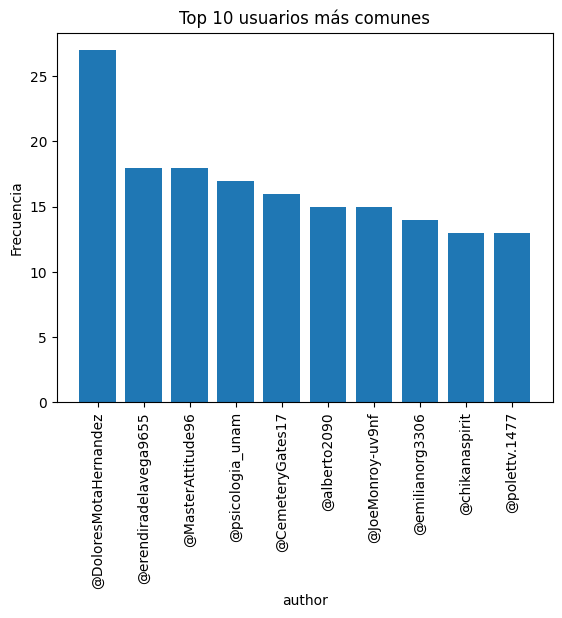
\includegraphics[width=14cm]{../Datos/Top10Usuarios}
	\caption{Top 10 de usuarios activos con mas comentarios durante el debate.}
	\label{fig:top10}
\end{figure}

En cuanto a la frecuencia de numero de votos, que un porcenpodemos observar que un porcentaje alto de los comentarios no presentan votos, mientras que un porcentaje alto de numero de votos entre 1 y 22 acumulan un alto porcentaje, pero no el mayor, en la figura \ref{fig:votosxreplicas} podemos identificar comentarios individuales con un alto numero de votos, los cuales son poco frecuentes pero muy significativos.\\


\begin{figure}[h!]
	\centering
	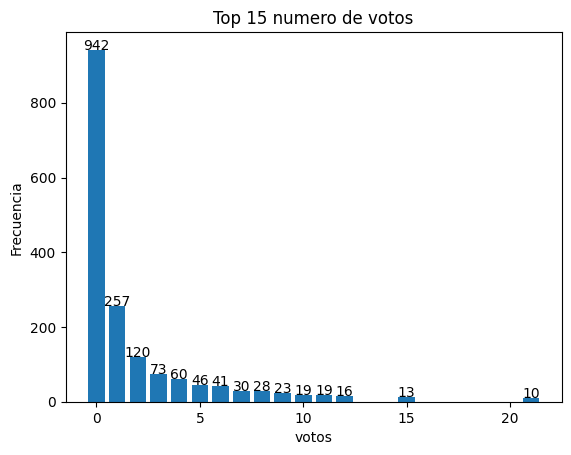
\includegraphics[width=14cm]{../Datos/Top10Votos}
	\caption{Top 10 del mayor numero frecuencia de votos en los comentarios.}
	\label{fig:top10V}
\end{figure}

En el comportamiento de las replicas podemos identificar una mayor frecuencia en un menor numero de replicas por comentario, es decir la gran mayoria de pocas replicas ocurren mas frecuentemente, al igual que la grafica anterior, podemos observar un comportamiento mas general en la figura \ref{fig:votosxreplicas}, donde se identifican la poca frecuencia de replicas continuas en en comentarios, es decir solo algunos comentarios son significativos y acumulan un alto numero de replicas.\\

\begin{figure}[h!]
	\centering
	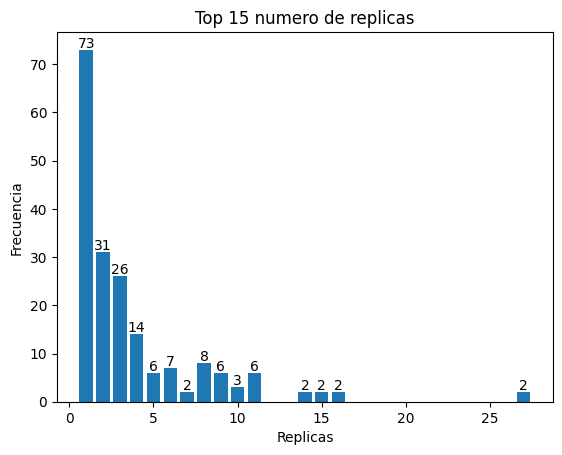
\includegraphics[width=13cm]{../Datos/Top10Replicas}
	\caption{Top 10 del mayor numero de frecuencias de replicas en los comentarios.}
	\label{fig:top10R}
\end{figure}


Al observar la distribución de votos Vs replicas de los comentarios, se puede identificar una relación entre los comentarios con mayor numero de votos y los comentarios con mayor numero de replicas, (ver figura \ref{fig:FyD}).\\


\begin{figure}[h!]
	\centering
	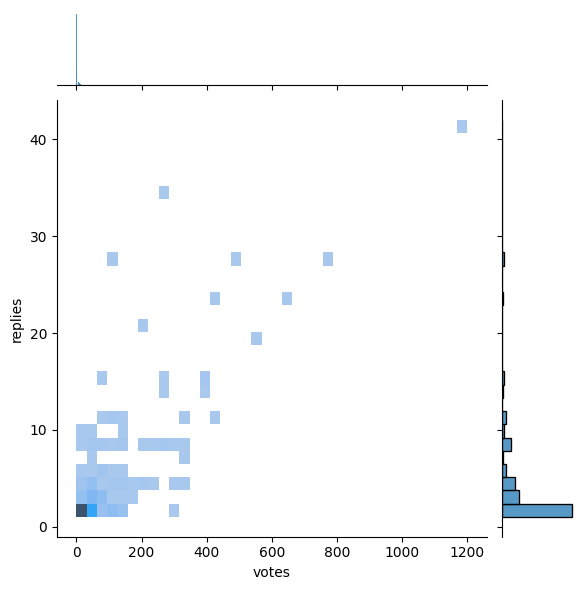
\includegraphics[width=11cm]{../Datos/AcumulacionYdistribuciones}
	\caption{grafico de frecuencias y distribución}
	\label{fig:FyD}
\end{figure}

\chapter{Procesado de los comentarios}

\section{Metodología}





\chapter{Conclusiones}

Según las encuestas y análisis publicados antes del primer debate presidencial en México 2024, las intenciones de voto se distribuían de la siguiente manera:

Claudia Sheinbaum (Morena, PT y PVEM): 49% (según encuesta “flash” publicada el 7 de abril de 2024)
Xóchitl Gálvez (PRI-PAN-PRD): 26% (según encuesta “flash” publicada el 7 de abril de 2024)
Jorge Álvarez Máynez (Movimiento Ciudadano): 18% (según encuesta “flash” publicada el 7 de abril de 2024)


La encuesta de El Financiero del 1 de abril de 2024 mostraba que Sheinbaum lideraba con un 35%, seguida de Gálvez con un 25% y Máynez con un 15%.

La encuesta de FactoMétrica y Reporte Índigo publicada el 9 de abril de 2024 mostraba que Sheinbaum lideraba con un 69%, seguida de Gálvez con un 26,5% y Máynez con un 4,5%.

La encuesta “flash” publicada el 7 de abril de 2024 mostraba que Sheinbaum lideraba con un 49%, seguida de Gálvez con un 26% y Máynez con un 18%.